\section{Introduction}

\subsection{Objectives} 

\begin{itemize}
\item Learn basic facts about the Karel language and its history. 
\item Learn how Karel differs from other programming languages.
\item Learn what skills this course provides.
\end{itemize}

\subsection{Brief history}

The educational programming language Karel the Robot was introduced by Richard E. 
Pattis in his book "Karel The Robot: A Gentle Introduction to the Art of Programming" in 1981. 
Pattis first used the language in his courses at Stanford University, and nowadays Karel is used at 
countless schools in the world. The language is named after Karel \v{C}apek, a Czech writer 
who invented the word "robot" in his 1921 science fiction play R.U.R. (Rossum's Universal Robots).

\subsection{Who is Karel?}

Karel is a little robot that lives in a maze and loves to collect gems.
He was manufactured with only five simple commands in his memory:

\begin{itemize}
\item {\color{blue} \tt go} ... make one step forward.
\item {\color{blue} \tt get} ... pick up a gem from the ground. 
\item {\color{blue} \tt left} ... turn to the left.
\item {\color{blue} \tt right} ... turn to the right. 
\item {\color{blue} \tt put} ... put a gem on the ground. 
\end{itemize}
He also has five built-in sensors that allow him to check his immediate surroundings:
\begin{itemize}
\item {\color{ForestGreen} \tt wall} ... true if he would crash into a wall by making one more step, false otherwise. 
\item {\color{ForestGreen} \tt gem} ... true if he stands on a gem, false otherwise.
\item {\color{ForestGreen} \tt north} ... true if he is facing North, false otherwise.
\item {\color{ForestGreen} \tt home} ... true if he is at home, false otherwise.
\item {\color{ForestGreen} \tt empty} ... true if his bag with gems is empty, false otherwise. 
\end{itemize}

\subsection{What will this course teach you?}

Computer programming skills are highly valued today, and they will be even more 
valued in the future. Karel is the perfect language for beginners. It will teach
you how to design algorithms and write working computer programs without struggling 
with technical complications of mainstream programming languages. Thanks to its 
simplicity, you should be done with Karel fairly quickly, and in no time you will be 
ready to move on to other programming languages. In particular, NCLab offers
Python programming: Textbook with exercises and review questions is available at 
{\tt http://femhub.com/textbook-python}). After finishing Karel, you will be able to 
transition to Python smoothly. 

\subsection{Is Karel a toy language?}

No, definitely not. Despite its playful appearance, Karel features all key
concepts of modern procedural programming. Computer programming includes two 
fairly independent tasks -- first to {\em design an algorithm} (sequence of 
steps leading to the solution of the problem at hand), and second, to {\em translate 
the algorithm into a suitable programming language}. The former skill is by 
far more important and therefore Karel puts maximum emphasis on it. This is 
why the language itself is kept so simple. As a matter of fact, the complexity 
of algorithms that you will encounter in this textbook ranges from trivial  
to extremely tough. Towards the end of the course you will encounter exercises
which you will probably not call toy problems.

\subsection{How does Karel differ from other programming languages?}

The biggest conceptual difference between Karel and mainstream procedural
programming languages such as Python, C, C++, Java or Fortran is that {\em 
the robot does not know math}. Math is not present in the first two levels
that correspond to the Pattis' book, and it is strongly suppressed in the 
advanced Level 3 as well. This is done for a reason -- math brings complications of its own 
which are unrelated to programming. In fact, many programming courses are
designed in such a way that students are struggling more with math than with 
programming. That's not good. Math (except for logic perhaps) is not needed to understand 
how to design great algorithms and to translate them into efficient computer 
programs. 
 
\section{Launching Karel}

\subsection{Objectives} 
\begin{itemize}
\item Learn to launch Karel and work with the graphical application.
\item Learn that Karel has several modes and how they differ.
\end{itemize}
\noindent
The simplest way to launch Karel is to click on the icon 
{\em Programming} and select {\em Karel} in the menu. This will launch the application 
in {\em Programming mode} with a randomly generated maze, as shown in Fig. \ref{fig:init}.

\begin{figure}[!ht]
\begin{center}
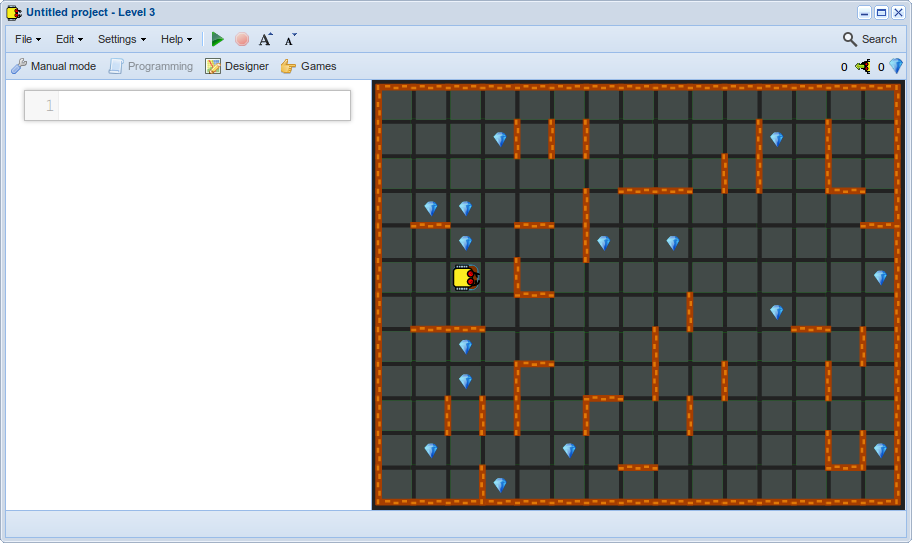
\includegraphics[width=0.7\textwidth]{img/init.png}
\end{center}
\vspace{-2mm}
\caption{Launching Karel in Programming mode, with a random maze.}
\label{fig:init}
%\vspace{-10mm}
\end{figure}

\noindent
The Programming mode is the most frequently used one. From there one can 
switch to {\em Manual mode}, {\em Designer mode}, and {\em Game mode} in 
the main menu. These modes will be discussed in more detail Paragraph \ref{levels}.

The application window contains the main menu on top,
work area on the left, maze on the right, and status bar on the bottom.
The menus are fairly intuitive, so let us explain just a few selected 
functions. In the {\em File} menu:

\begin{itemize}
\item {\em Open} will open a Karel file that you created and saved, or cloned previously.
\item {\em Clone} will help you search and download public Karel projects from the database. 
\item {\em Add static URL} will create a HTML address for your project. Such a link can be 
      included in any web page. 
\end{itemize}
The {\em Maze} menu facilitates operating with mazes, including creating a new random 
one, duplicating an existing maze, restoring maze to its saved version, and save and remove 
maze. The {\em Edit} menu enables operation with code and text cells (to be discussed in 
Section \ref{sec:editmenu}). In {\em Settings} one can change Karel's Level, change his 
speed, and adjust sound preferences. 

The green and red 
buttons are used to run and stop programs, respectively, and the two buttons next to them on
the right can be used to increase and decrease font size. The pair of icons on far right is the 
step counter (that can be reset by clicking on it) and gem counter that indicates how many gems 
Karel has in his bag.

\subsection{Karel modes} \label{levels}

Karel operates in four modes:
\begin{itemize}
\item {\em Manual mode:} The robot is controlled using the mouse and five buttons Go, Get, Left, Right, and Put. 
      Watch out and do not crash!
\item {\em Programming mode:} The robot is controlled using written programs (computer code). This mode has 
      three Levels:
\begin{itemize}
\item Level 1 serves as transition layer between the Manual and Programming modes. Programs are written using only 
      five commands {\tt go}, {\tt get}, {\tt left}, {\tt right}, and {\tt put} that exactly correspond to 
      the buttons Go, Get, Left, Right, and Put in Manual mode.
\item Level 2 is where the actual programming begins. On top of the commands from Level 1, programs can contain 
      conditions, loops, and custom commands.
\item Level 3 goes beyond the original Pattis' book by introducing variables, lists, and functions that 
      return values. In this level Karel also gets a GPS device that allows him to determine his position 
      in the maze. The functionality of Level 3 can be used to design entry-level artificial 
      intelligence (AI) algorithms. 
\end{itemize}
\item {\em Designer mode} allows the user to create custom mazes.
\item {\em Game mode} makes it possible to create and play games. 
\end{itemize}

%%%%%%%%%%%%%%%%%%%%%%%%%%%%%%%%%%%%%%%%%%%%%%%%%%%%%%%%%%%%%%%%%%%%%%%%%%%%%%%

\section{Manual Mode} \label{sec:manual}

\subsection{Objectives} 
\begin{itemize}
\item Learn to operate the robot in Manual mode.
\end{itemize}
\noindent
Before we begin, let us review the four directions on the compass:\\[-7mm]

\begin{figure}[!ht]
\begin{center}
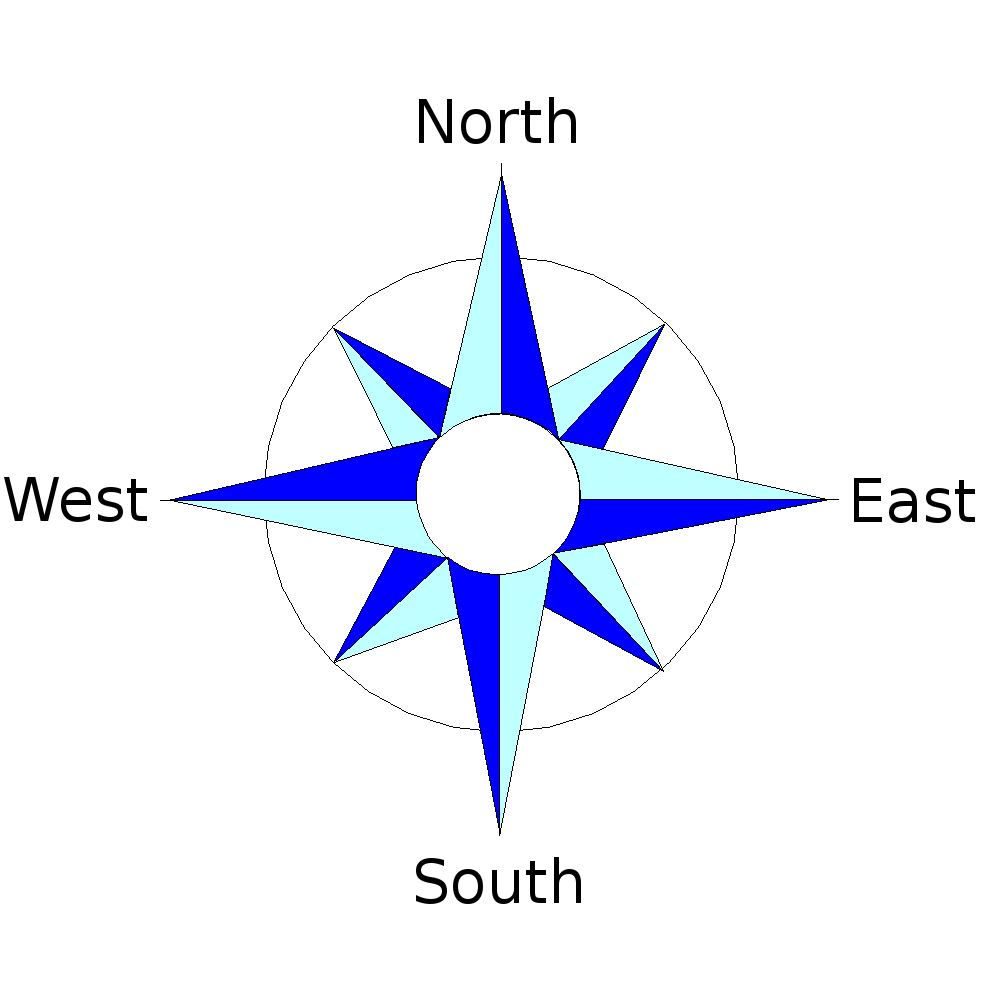
\includegraphics[width=0.35\textwidth]{img/compass.png}
\vspace{-0mm}
%\caption{Karel's four possible orientations.}
%\label{fig:ori}
\end{center}
\vspace{-1cm}
\end{figure}

\noindent
When launching Karel through the Programming icon, switch to Manual mode using the corresponding 
menu button. Then, five buttons Left, Right, Go, Get and Put will appear in the panel on the left,
as shown in Fig. \ref{fig:buttons}.

\begin{figure}[!ht]
\begin{center}
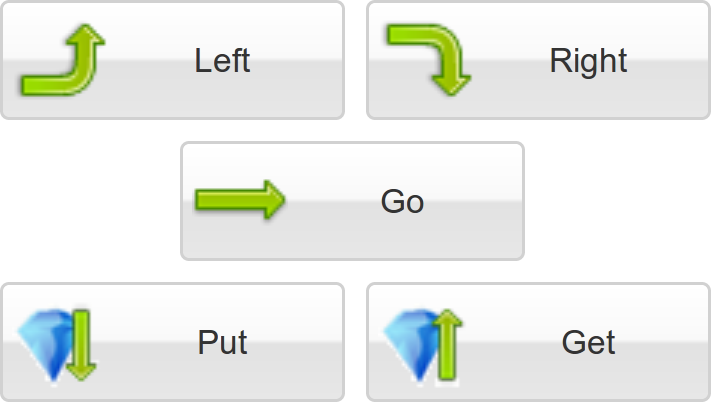
\includegraphics[width=6.2cm]{img/buttons-all.png}
\vspace{-0mm}
\caption{Karel's buttons in Manual mode (robot facing East).}
%\vspace{-1cm}
\label{fig:buttons}
\end{center}
\end{figure}
\noindent
The function of the buttons is self-explanatory -- pressing Left will turn the robot 90 degrees to the left,
pressing Right will turn him 90 degrees to the right, and pressing Go will move him one step forward 
(watch out and do not crash!). Upon pressing Put the robot will reach into his bag with gems, 
take one, and put it on the ground where he stands. 
An indicator showing how many gems are in the bag can be found in the upper right 
corner of the window. Last, upon pressing 
Get the robot will pick up a gem from the ground where he stands. If 
one asks the robot to get a gem where there is none, he will complain.

When the robot turns, the arrows on the buttons adjust automatically to his new 
direction. This is illustrated in Fig. \ref{fig:buttons2}.

\begin{figure}[!ht]
\begin{center}
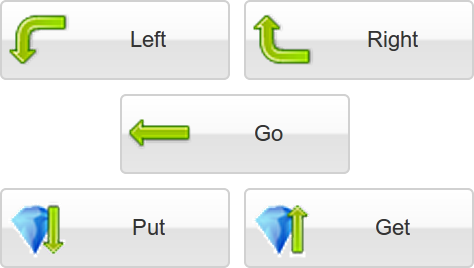
\includegraphics[width=6.2cm]{img/buttons-all-2.png}
\vspace{-0mm}
\caption{Karel's buttons in Manual mode (robot facing West).}
\label{fig:buttons2}
\end{center}
\end{figure}

%%%%%%%%%%%%%%%%%%%%%%%%%%%%%%%%%%%%%%%%%%%%%%%%%%%%%%%%%%%%%%%%%%%%%%%%%%%%%%%

\section{Programming Mode} \label{sec:bridge}

\subsection{Objectives} 
 
\begin{itemize}
\item Start operating the robot in Programming mode.
\item Understand the difference between {\em algorithm} and {\em program}. 
\item Learn the difference between {\em syntactical} and {\em logical} mistakes.
\item Understand that {\em debugging} is an indivisible part of computer programming.
\end{itemize}

\subsection{Typing commands}
In Programming mode, commands for the robot are entered into an code cell located in the left panel.
These commands are {\tt left}, {\tt right}, {\tt go}, {\tt get}, and {\tt put}.
Their function is the same as the function of the corresponding buttons in Manual mode.
One or more commands form a {\em computer program (computer code)}. Often 
we just say {\em program} or {\em code}.
There are two simple rules to remember:
\begin{enumerate}
\item Always type one command per line.
\item Do not enter empty characters in front of commands. 
\end{enumerate}
Ignoring these rules would not make the program invalid, but the code would be 
difficult to read. It is important to write a clean, transparent code. 

\subsection{Algorithms, programs, and bugs} \label{subsec:interm1}

Karel always obeys all commands {\em exactly}. Sometimes it may happen that 
we plan one thing but to our surprise the robot does something else. In most cases this 
happens when our {\em algorithm} is wrong. By an {\em algorithm} we mean a sequence of 
logical steps that the robot needs to follow in order to fulfill his task. Algorithms 
are presented using normal human language, not in terms of the robot's commands. 

{\em Program} or {\em computer code} is created when the algorithm is expressed
in terms of the robot's language. When our algorithm is good, then 
the program is easy to write.

Mistakes in algorithms are called {\em logical errors}. A logical error is, for 
example, when we crash the robot into a wall because we forgot to make a turn.
Mistakes such as mis-spelling a command, writing "1o" instead of "10", or forgetting 
indentation are related to 
{\em syntax} and they are called {\em syntactical errors}. Of these two types, 
logical errors are usually much more difficult to find. 

In general, mistakes or either kind are called {\em bugs} and the procedure of 
eliminating them is called {\em debugging}. Depending on how careful we 
were while preparing our algorithm and writing the program, debugging takes either 
a short time or a long time. It does not happen often that a program works correctly
right away. 

When we commit a syntactical error,
the robot will write an error message and do nothing.
If our algorithm contains a logical error, then he will
write an error message and stop executing the program. 
The most usual logical error are:

\begin{itemize}
\item Karel crashes into a wall.
\item The robot tries to collect a gem where is none.
\item He attempts to put a gem on the ground while his bag is empty.
\end{itemize}

%%%%%%%%%%%%%%%%%%%%%%%%%%%%%%%%%%%%%%%%%%%%%%%%%%%%%%%%%%%%%%%%%%%%%%%%%%%%%%%

\section{Counting Loop} \label{sec:repeat}

\subsection{Objectives} 

\begin{itemize}
\item Learn to make the robot repeat something a given number of times.
\end{itemize}

\noindent
In Section \ref{sec:bridge} we successfully crossed the bridge between manual control 
and programming. The bridge collapsed, there is no way back. But do 
not worry about that! The land of Programming is much more beautiful,
and once you understand its beauty, you will never want to leave.

\subsection{The {\tt repeat} command}

The {\em counting loop}, represented by the {\tt repeat} command, can save 
us lots of writing when something is repeated a given number of times. 
For example, for Karel to make 15 steps forward we could type:\\

\begin{bbox}
\begin{Verbatim}[commandchars=\\\{\}]
\PY{n+nf}{go}
\PY{n+nf}{go}
\PY{n+nf}{go}
\PY{n+nf}{go}
\PY{n+nf}{go}
\PY{n+nf}{go}
\PY{n+nf}{go}
\PY{n+nf}{go}
\PY{n+nf}{go}
\PY{n+nf}{go}
\PY{n+nf}{go}
\PY{n+nf}{go}
\PY{n+nf}{go}
\PY{n+nf}{go}
\PY{n+nf}{go}
\end{Verbatim}
\end{bbox}
\vspace{6mm}

\noindent
But this is neither efficient nor elegant. Instead, the same can be
achieved by telling Karel to {\tt repeat} the {\tt go} command {\tt 15} times:\\

\begin{bbox}
\begin{Verbatim}[commandchars=\\\{\}]
\PY{k}{repeat} 15
    \PY{n+nf}{go}
\end{Verbatim}
\end{bbox}
\vspace{6mm}

\noindent
There are a few simple rules that we need to remember when using the {\tt repeat} command:

\begin{itemize}
\item Keep code readable -- always write one command per line.
\item Indentation -- all commands to be repeated (the {\em body of the loop}) need to be indented. 
      One can choose between 2-indent and 4-indent. The former yields more compact 
      code with not-so-long lines, the latter is easier to read. 
\item Cancel the indentation for the first command that does not belong to the body of the loop.
\end{itemize}
To illustrate what the indentation does, let's look at a code that will move the robot 8 steps forward:\\

\begin{bbox}
\begin{Verbatim}[commandchars=\\\{\}]
\PY{k}{repeat} 4
    \PY{n+nf}{go}
    \PY{n+nf}{go}
\end{Verbatim}
\end{bbox}
\vspace{6mm}

\noindent
Compare to a code that will only move the robot 5 steps forward:\\

\begin{bbox}
\begin{Verbatim}[commandchars=\\\{\}]
\PY{k}{repeat} 4
    \PY{n+nf}{go}
\PY{n+nf}{go}
\end{Verbatim}
\end{bbox}
\vspace{6mm}

\noindent
Multiple {\tt repeat} commands can be {\em nested}. This means that a {\tt repeat} command 
can used in the body of another {\tt repeat} command. Everything that was said about indentation 
still holds. Can you figure out what the following code does?\\

\begin{bbox}
\begin{Verbatim}[commandchars=\\\{\}]
\PY{k}{repeat} 10
    \PY{k}{repeat} 5
        \PY{n+nf}{go}
    \PY{k}{repeat} 2
        \PY{n+nf}{left}
\end{Verbatim}
\end{bbox}
\vspace{6mm}

\noindent
After you figured it out, launch Karel via the {\em Programming} menu, enter this code into
the code cell, and run it! But before doing that, remember to switch to {\em Designer} and make 
some free space in front of the robot 
so that he does not crash into a wall.


\section{Working with Code and Text Cells} \label{sec:editmenu}

\subsection{Objectives} 
 
\begin{itemize}
\item Learn why it is good to include comments in the code.
\item Learn how to add new code cells and descriptive text cells.
\item Learn how to change the order of cells.
\item Learn how to run all code cells at once, and how to run them individually.
\item Learn how to clear, collapse, remove and merge cells.
\end{itemize}
It is a very good habit to add comments to programs (every line starting with the '{\tt \#}'
symbol is a comment) and also to include descriptive 
texts in Karel worksheets, since descriptions make it easier for someone else to 
understand your program. Sometimes you may be in the position of the "someone else" yourself,
when you return to your own program some time after you wrote it. Here are a couple of 
simple new rules to remember:
\begin{enumerate} 
\item New text cell can be added under the current cell via the button 
      {\em Add text cell} under the cell. 
      After an empty text cell appears, click into it and add text. The text can be 
      formatted and/or colors using the menu. After you are finished, click 
      on the button {\em Save cell} under the text cell. 
\item New code cell can be added under a cell by clicking on {\em Add code cell} 
      under the cell. Having multiple code cells can be useful, for example, to test various versions 
      of our program, or if we want to run parts of the program separately. 
\item Order of cells can be changed via the arrows under the cells.
\item Clicking on {\em Clear cell} under a cell will erase its contents.
\item Any cell can be collapsed by clicking on the {\em Collapse cell} button
      under the cell. Then a new button {\em Expand this cell} will appear instead
      of the original cell. The cell can be expanded by clicking on this button.
\item Clicking on the button {\em Remove cell} under a cell will remove it. 
      All text or code in that cell will be lost.
\item Run programs via the green arrow button in the main menu (this will evaluates all code
      cells). Each cell can be also evaluated individually by clicking on the green 
      arrow button under the cell. If there is just one code cell, both options 
      are equivalent.
\item Programs can be stopped using the red button in the menu. 
\item If a particular
      code cell needs to be stopped, then use the red button under that cell.
\item Cells can be merged via the options {\em Merge active cell up} and 
      {\em Merge active cell down} in Edit menu.
\end{enumerate}

%%%%%%%%%%%%%%%%%%%%%%%%%%%%%%%%%%%%%%%%%%%%%%%%%%%%%%%%%%%%%%%%%%%%%%%%%%%%%%%

\section{Conditions} \label{sec:cond}

\subsection{Objectives} 

\begin{itemize}
\item Understand the function of Karel's five sensors.
\item Learn to use the sensors in conjunction with {\em conditions} to help Karel 
      check his surroundings and react accordingly. For example, we will learn to first 
      check whether wall is ahead before making a step forward, checking whether there
      is a gem on the ground before attempting to pick it up, etc.
\end{itemize}

\noindent
Karel has built-in sensors to better navigate in the maze:

\subsection{Karel's five sensors}

\noindent
\underline{{\tt wall} sensor}

The first one is an infrared sensor {\tt wall} that the robot uses to determine 
whether it is safe to make one step forward, or whether there is a wall. This is 
illustrated in Fig. \ref{fig:dede-ifelse}.
\begin{figure}[!ht]
\begin{center}
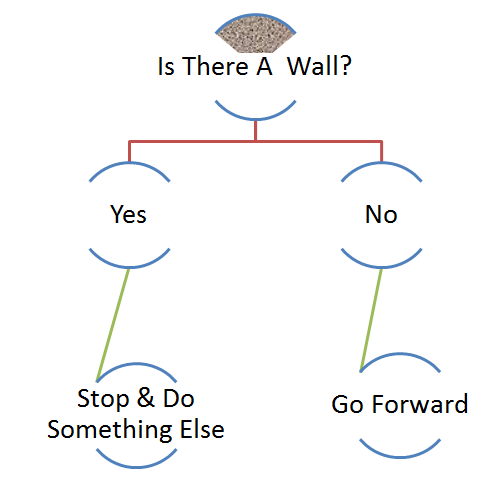
\includegraphics[height=0.4\textwidth]{img/salih-ifelse.png}
\end{center}
\vspace{-4mm}
\caption{This is how Karel uses the {\tt wall} sensor!}
\label{fig:dede-ifelse}
%\vspace{-10mm}
\end{figure}

\noindent
The usage of the {\tt wall} sensor in a program can be illustrated using a simple program "Careful step" 
where Karel first checks whether there is a wall ahead before
making a step. If there is wall, he turns back:\\

\begin{bbox}
\begin{Verbatim}[commandchars=\\\{\}]
\PY{c}{\PYZsh{} Program "Careful step".}
\PY{k}{if} \PY{n+nb+bp}{wall}
    \PY{k}{repeat} 2
        \PY{n+nf}{left}
\PY{k}{else}
    \PY{n+nf}{go}
\end{Verbatim}
\end{bbox}
\vspace{6mm}

\noindent
As we mentioned before, the symbol '{\tt \#}' introduces a comment, meaning that the line 
of code behind it is ignored by the robot.
The {\tt else} branch does not have to be there if it is not needed. Notice the indentation 
of the bodies of the {\tt if} and {\tt else} branches - this is analogous 
to how we indent the body of the {\tt repeat} command. There are four more sensors:\\

\noindent
\underline{{\tt gem} sensor} returns true if the robot stands on a gem, false otherwise. \\

\noindent
\underline{{\tt empty} sensor} returns true if the robot's bag with gems is empty, false otherwise. \\

\noindent
\underline{{\tt north} sensor} returns true if the robot is facing North, false otherwise.\\

\noindent
\underline{{\tt home} sensor} returns true if the robot is at home, false otherwise.

\subsection*{Testing opposites}

Karel can also use the reserved word {\tt not} to test the opposites.
For illustration, the previous program can be rewritten as follows, without 
changing its function:\\

\begin{bbox}
\begin{Verbatim}[commandchars=\\\{\}]
\PY{c}{\PYZsh{} Program "Careful step".}
\PY{k}{if} \PY{n+nb+bp}{not} \PY{n+nb+bp}{wall}
    \PY{n+nf}{go}
\PY{k}{else}
    \PY{k}{repeat} 2
        \PY{n+nf}{left}
\end{Verbatim}
\end{bbox}
\vspace{6mm}

\noindent

\subsection{Programming hints}

Good programmer is a careful programmer! Errors can be avoided by always checking the 
appropriate sensor before making an action. A few examples of careful actions:\\
 
\begin{bbox}
\begin{Verbatim}[commandchars=\\\{\}]
\PY{k}{if} \PY{n+nb+bp}{not} \PY{n+nb+bp}{wall}
    \PY{n+nf}{go}
\end{Verbatim}
\end{bbox}
\vspace{6mm}

\noindent
Another example:\\
 
\begin{bbox}
\begin{Verbatim}[commandchars=\\\{\}]
\PY{k}{if} \PY{n+nb+bp}{gem}
    \PY{n+nf}{get}
\end{Verbatim}
\end{bbox}
\vspace{6mm}

\noindent
And one more:\\
 
\begin{bbox}
\begin{Verbatim}[commandchars=\\\{\}]
\PY{k}{if} \PY{n+nb+bp}{not} \PY{n+nb+bp}{empty}
    \PY{n+nf}{put}
\end{Verbatim}
\end{bbox}
\vspace{6mm}

\noindent

%%%%%%%%%%%%%%%%%%%%%%%%%%%%%%%%%%%%%%%%%%%%%%%%%%%%%%%%%%%%%%%%%%%%%%%%%%%%%%%

\section{Conditional Loop} \label{sec:whilek}

\subsection{Objectives} 
 
\begin{itemize}
\item Learn to repeat a command or a sequence of commands when it is not known 
      how many repetitions will be needed.
\end{itemize}

\subsection{The {\tt while} command}

Often Karel needs to repeat something, {\em not knowing in advance how many repetitions
there will be}. So, the {\tt repeat} command is not practical. This can be the case, for example, 
when the robot is asked to walk straight ahead until he reaches the closest wall.
Remember that he only can see walls that are right ahead of him -- walls 
that are further away he can't see. Such a program would be:\\

\begin{bbox}
\begin{Verbatim}[commandchars=\\\{\}]
\PY{k}{while} \PY{n+nb+bp}{not} \PY{n+nb+bp}{wall}
    \PY{n+nf}{go}
\end{Verbatim}
\end{bbox}
\vspace{6mm}

\noindent
Or, Karel may be asked to walk until he gets home:\\

\begin{bbox}
\begin{Verbatim}[commandchars=\\\{\}]
\PY{k}{while} \PY{n+nb+bp}{not} \PY{n+nb+bp}{home}
    \PY{n+nf}{go}
\end{Verbatim}
\end{bbox}
\vspace{6mm}

\noindent
Beware though: {\color{red}{this program is dangerous}} since the robot will crash into a wall
if his home is not straight ahead of him!\\

\noindent
The robot may be asked to empty his bag (he does not know how many gems are in it):\\
 
\begin{bbox}
\begin{Verbatim}[commandchars=\\\{\}]
\PY{k}{while} \PY{n+nb+bp}{not} \PY{n+nb+bp}{empty}
    \PY{n+nf}{put}
\end{Verbatim}
\end{bbox}
\vspace{6mm}

\noindent
Or, he may be asked to collect all gems from a pile (he does not know 
how many gems there are):\\

\begin{bbox}
\begin{Verbatim}[commandchars=\\\{\}]
\PY{k}{while} \PY{n+nb+bp}{gem}
    \PY{n+nf}{get}
\end{Verbatim}
\end{bbox}
\vspace{6mm}

\noindent
Or we may ask him to turn to face North (recall that the robot does not know which direction he is
facing - there is no such sensor):\\

\begin{bbox}
\begin{Verbatim}[commandchars=\\\{\}]
\PY{k}{while} \PY{n+nb+bp}{not} \PY{n+nb+bp}{north}
    \PY{n+nf}{left}
\end{Verbatim}
\end{bbox}
\vspace{6mm}

\noindent
At last, let us write the following program: Karel is asked to 
turn South, walk straight ahead until he reaches the closest wall, and 
collect all gems that he can find on the way:

\begin{bbox}
\begin{Verbatim}[commandchars=\\\{\}]
\PY{c}{\PYZsh{} First turn North.}
\PY{k}{while} \PY{n+nb+bp}{not} \PY{n+nb+bp}{north}
    \PY{n+nf}{left}

\PY{c}{\PYZsh{} Then turn South.}
\PY{k}{repeat} 2
    \PY{n+nf}{left}

\PY{c}{\PYZsh{} Go straight ahead and pick all gems.}
\PY{k}{while} \PY{n+nb+bp}{not} \PY{n+nb+bp}{wall}
    \PY{k}{if} \PY{n+nb+bp}{gem}
        \PY{n+nf}{get}
    \PY{n+nf}{go}

\PY{c}{\PYZsh{} Pick gem at the wall (if any).}
\PY{k}{if} \PY{n+nb+bp}{gem}
    \PY{n+nf}{get}
\end{Verbatim}
\end{bbox}
\vspace{6mm}

\noindent
Notice that we first need to turn the robot to face North -- this is because North 
is the only direction that he can check!


%%%%%%%%%%%%%%%%%%%%%%%%%%%%%%%%%%%%%%%%%%%%%%%%%%%%%%%%%%%%%%%%%%%%%%%%%%%%%%%

\section{Custom Commands} \label{sec:newcom}

\subsection{Objectives} 
 
\begin{itemize}
\item Learn that replicating computer code is a bad habit.
\item Learn that splitting the big task into smaller ones will simplify the solution a lot. 
\item Learn to bring more structure and clarity into our programs by introducing new commands.
\end{itemize}

\subsection{Programming hints}

{\em Always look for small tasks that can be solved independently of the big ones.
Solve the small tasks first, and you will see that the big ones get much simpler. The 
importance of what we just said cannot be stressed more.}\\

\noindent
The fact that you are reading this line of text proves that you are not 
a perfect programmer yet. A perfect programmer would be stuck forever 
in the previous three lines which are an infinite loop!

%\begin{figure}[!ht]
%\begin{center}
%
\includegraphics[width=0.2\textwidth]{img/smiley.png}
%\end{center}
%\vspace{-1cm}
%\end{figure}

\subsection{Never replicate computer code}

A new command should be defined whenever it becomes clear that the same 
action is repeated in the algorithm multiple times (yes, we talk about the algorithm,
not about the program). When we start writing a program and then realize that the same
code repeats itself at various places, then probably we did not do a good job 
designing the algorithm.

Sometimes it might be 
tempting to just replicate the same code several times in the 
program, because it does the same thing, but do not do it! This would be very bad programming
and sooner or later our own code would punish us for that. 
We would make a small change at one place but forget to do it 
in all the other places. Then our code would start 
acting strange, it would sometimes work and sometimes fail. 
We would spend lots of time looking for the mistakes, find some 
of them but not all, and our program would become unreliable
and after some time irreparable. We would find that we need to 
rewrite it from scratch.

\subsection{Defining new commands}

New commands are defined using the reserved word 
{\tt def}. For example, in a program where the robot needs to turn back
many times, it is a good idea to define a new command {\tt back}
as follows:\\

\begin{bbox}
\begin{Verbatim}[commandchars=\\\{\}]
\PY{k}{def} back
    \PY{k}{repeat} 2
        \PY{n+nf}{left}
\end{Verbatim}
\end{bbox}
\vspace{6mm}

\noindent
Note the indent -- the body of a new command needs to be indented 
analogously to the bodies of loops and conditions.

%%%%%%%%%%%%%%%%%%%%%%%%%%%%%%%%%%%%%%%%%%%%%%%%%%%%%%%%%%%%%%%%%%%%%%%%%%%%%%%

\section{Recursion} \label{sec:recursion}

\subsection{Objectives} 
 
\begin{itemize}
\item Understand what recursion is and when it can be useful.
\item Learn to write good recursive algorithms.
\end{itemize}
By a {\em recursive} algorithm we mean an algorithm that makes a call to itself. How does it sound?
In our life we use recursion all the time, without noticing it. For example, when we descend 
a staircase, our algorithm is:\\

\begin{bbox}
\begin{Verbatim}[commandchars=\\\{\}]
Descend_staircase
    Descend_one_step
    If this_was_not_the_last_step
        Descend_staircase
\end{Verbatim}
\end{bbox}
\vspace{6mm}

\noindent
Recursion is not applicable to all types of problems, but it can be very 
helpful, especially for problems where we can
\begin{itemize}
\item reduce the problem to a similar one which is smaller in size, 
\item apply the same algorithm to the smaller problem. 
\end{itemize}
On program level, this means that some command calls itself, either 
directly or through other commands.

\subsection[\ \ How it works]{How it works} 

Consider the following Karel program:\\

\begin{bbox}
\begin{Verbatim}[commandchars=\\\{\}]
\PY{k}{def} reach_wall
    \PY{k}{if} \PY{n+nb+bp}{not} \PY{n+nb+bp}{wall}
        \PY{n+nf}{go}
        reach_wall

reach_wall
\end{Verbatim}
\end{bbox}
\vspace{6mm}

\noindent
Imagine that the initial position of the robot is like in Fig. \ref{fig:rec1}.


\begin{figure}[!ht]
\begin{center}
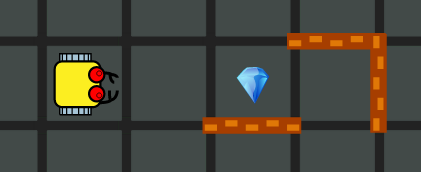
\includegraphics[width=6cm]{img/rec-1.png}
\end{center}
\vspace{-4mm}
\caption{Robot's initial position.}
\label{fig:rec1}
\vspace{-4mm}
\end{figure}
\noindent
When the command {\tt reach\_wall} is first called, the robot stands three steps away from the wall and 
thus the {\tt if not wall} condition passes. Then the command {\tt go} follows and the robot's 
position changes as shown in Fig. \ref{fig:rec2}. 

\begin{figure}[!ht]
\begin{center}
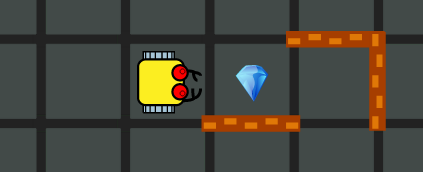
\includegraphics[width=6cm]{img/rec-2.png}
\end{center}
\vspace{-4mm}
\caption{Robot's position after making the first step forward.}
\label{fig:rec2}
\vspace{-4mm}
\end{figure}
\noindent
Next the robot executes the {\tt reach\_wall} command that follows the {\tt go} command. A good way to 
understand what happens is to imagine that the command is replaced with its own body. So the corresponding 
code would look as follows:\\

\begin{bbox}
\begin{Verbatim}[commandchars=\\\{\}]
\PY{k}{if} \PY{n+nb+bp}{not} \PY{n+nb+bp}{wall}
    \PY{n+nf}{go}
    \PY{k}{if} \PY{n+nb+bp}{not} \PY{n+nb+bp}{wall}
        \PY{n+nf}{go}
        reach_wall
\end{Verbatim}
\end{bbox}
\vspace{6mm}

\noindent
Since the robot is two steps away from the wall, the second {\tt if not wall} condition passes and 
he makes a second step forward. His new position is shown in Fig. \ref{fig:rec3}.

\begin{figure}[!ht]
\begin{center}
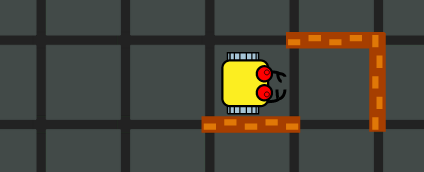
\includegraphics[width=6cm]{img/rec-3.png}
\end{center}
\vspace{-4mm}
\caption{Robot's position after making the second step forward.}
\label{fig:rec3}
\vspace{-4mm}
\end{figure}
\noindent
Next the robot executes the third {\tt reach\_wall} command. Again we can imagine that the command 
is replaced with its own body. The corresponding code would look as follows:\\

\begin{bbox}
\begin{Verbatim}[commandchars=\\\{\}]
\PY{k}{if} \PY{n+nb+bp}{not} \PY{n+nb+bp}{wall}
    \PY{n+nf}{go}
    \PY{k}{if} \PY{n+nb+bp}{not} \PY{n+nb+bp}{wall}
        \PY{n+nf}{go}
        \PY{k}{if} \PY{n+nb+bp}{not} \PY{n+nb+bp}{wall}
            \PY{n+nf}{go}
            reach_wall
\end{Verbatim}
\end{bbox}
\vspace{6mm}

\noindent
Since the robot is one step away from the wall, the third {\tt if not wall} condition passes and 
he makes a third step forward. His new position is shown in Fig. \ref{fig:rec4}.

\begin{figure}[!ht]
\begin{center}

\includegraphics[width=6cm]{img/rec-4.png}
\end{center}
\vspace{-4mm}
\caption{Robot's position after making the third step forward.}
\label{fig:rec4}
%\vspace{-10mm}
\end{figure}
\noindent
Now the robot stands in front of the wall, so it gets more interesting. The 
{\tt reach\_wall} command is executed one more time, so we can imagine that its body 
is pasted into the code one last time:\\

\begin{bbox}
\begin{Verbatim}[commandchars=\\\{\}]
\PY{k}{if} \PY{n+nb+bp}{not} \PY{n+nb+bp}{wall}
    \PY{n+nf}{go}
    \PY{k}{if} \PY{n+nb+bp}{not} \PY{n+nb+bp}{wall}
        \PY{n+nf}{go}
        \PY{k}{if} \PY{n+nb+bp}{not} \PY{n+nb+bp}{wall}
            \PY{n+nf}{go}
            \PY{k}{if} \PY{n+nb+bp}{not} \PY{n+nb+bp}{wall}
                \PY{n+nf}{go}
                reach_wall
\end{Verbatim}
\end{bbox}
\vspace{6mm}

\noindent
However, now the {\tt if not wall} condition does not pass, which means that  
the program is finished!

\subsection[\ \ The base case]{The base case}

In the last example we have observed one important fact: To prevent infinite recursion, we 
used an {\tt if} statement. The {\tt else} statement was omitted which meant "else do nothing".
In recursive algorithms, we always need an {\tt if} or {\tt if-else} statement of some sort, 
where one branch makes a recursive call while the other one does not. 
The branch without a recursive call is called the {\em base case}. A bad example 
of a recursive command without a base case would be\\

\begin{bbox}
\begin{Verbatim}[commandchars=\\\{\}]
\PY{k}{def} left_forever
    \PY{n+nf}{left}
    left_forever
\end{Verbatim}
\end{bbox}
\vspace{6mm}

\noindent
This program is an infinite recursion that needs to be stopped using the 
red stop button.

\subsection[\ \ When should recursion be used?]{When should recursion be used?}

The recursive command {\tt reach\_wall} that we defined above may not be the most useful example 
since the same functionality could be achieved more elegantly without recursion, just with\\

\begin{bbox}
\begin{Verbatim}[commandchars=\\\{\}]
\PY{k}{def} reach_wall
    \PY{k}{while} \PY{n+nb+bp}{not} \PY{n+nb+bp}{wall}
        \PY{n+nf}{go}
\end{Verbatim}
\end{bbox}
\vspace{6mm}

\noindent
If there is a small task that needs to be solved repeatedly in order to get a bigger task done,
then often one can write both a non-recursive and recursive version. Recall for example the Diamond
Staircase example from Section \ref{sec:newcom}. The small task there was to climb one step and pick 
up the gem, ending up facing east. A non-recursive version of the algorithm would be:\\

\begin{bbox}
\begin{Verbatim}[commandchars=\\\{\}]
\PY{k}{def} climb_one_step
    \PY{n+nf}{left}
    \PY{n+nf}{go}
    \PY{n+nf}{right}
    \PY{n+nf}{go}
    \PY{n+nf}{get}

\PY{k}{while} \PY{n+nb+bp}{not} \PY{n+nb+bp}{home}
    climb_one_step
\end{Verbatim}
\end{bbox}
\vspace{6mm}

\noindent
A recursive version of the same:\\

\begin{bbox}
\begin{Verbatim}[commandchars=\\\{\}]
\PY{k}{def} climb_the_stairs
    \PY{k}{if} \PY{n+nb+bp}{not} \PY{n+nb+bp}{home}
        \PY{n+nf}{left}
        \PY{n+nf}{go}
        \PY{n+nf}{right}
        \PY{n+nf}{go}
        \PY{n+nf}{get}
        climb_the_stairs

climb_the_stairs
\end{Verbatim}
\end{bbox}
\vspace{6mm}

\noindent
If an algorithm comes in both a recursive and a non-recursive version, then the following 
should be taken into account:
\begin{itemize}
\item The recursive version will be slightly slower than a non-recursive one. The reason is 
      the overhead related to creating a new instance of the recursive command and calling it. 
\item The recursive version will also require more memory -- when a recursive command is called 
      1000 times, then it actually exists in 1000 copies in the memory. Hence, recursion is 
      not recommended with very large numbers of repetitions.
\end{itemize}
Recursive algorithms are used mainly where non-recursive ones are cumbersome to design. 
For example, much code written for traversing tree-like data structures is recursive. Also certain 
sorting algorithms are more naturally written in recursive form. We will discuss these subjects 
in more detail later.

\subsection[\ \ Mutually recursive commands]{Mutually recursive commands}

Recursion can have interesting forms. For example, there can be a pair of commands
that call themselves mutually, such as the commands {\tt odd} and 
{\tt even} in the following example (that also solves the Diamond Staircase
problem). Note the presence of base case in both recursive commands:\\
 
\begin{bbox}
\begin{Verbatim}[commandchars=\\\{\}]
\PY{k}{def} climb_step
    \PY{n+nf}{left}
    \PY{n+nf}{go}
    \PY{n+nf}{right}
    \PY{n+nf}{go}
    \PY{n+nf}{get} 

\PY{k}{def} odd
    \PY{k}{if} not home
        climb_step
        even

\PY{k}{def} even
    \PY{k}{if} not home
        climb_step
        odd
    
odd
\end{Verbatim}
\end{bbox}

%%%%%%%%%%%%%%%%%%%%%%%%%%%%%%%%%%%%%%%%%%%%%%%%%%%%%%%%%%%%%%%%%%%%%%%%%%%%%%%

\section{Variables and Functions} \label{sec:var}

In this Section we are entering exciting Level 3 where Karel grows up and leaves the 
home of his parents to experience life on his own. Therefore, his home will not be 
present in the maze anymore. There are additional changes
that reflect Karel's growing up -- there is a GPS device that Karel can use to 
determine his position in the maze, he can print messages, work with variables and 
lists, employ functions that return values, and more. Do not forget to switch to 
Level 3 in Settings. A compact overview of new functionality in Level 3 can be found 
in Section \ref{sec:newfunc3}.

\subsection[\ \ Objectives]{Objectives} 
 
\begin{itemize}
\item Understand the concept of variables.
\item Learn to work with numerical and logical variables and text strings.
\item Learn to use functions that return values. 
\item Understand that variables defined inside functions are local. 
\end{itemize}

\noindent
In programming, variables are used to store useful information for later use. 
To give a few examples, this information can be a number, word, sentence, 
or a logical value ("true" or "false").

\subsection[\ \ Types of variables]{Types of variables}

All of us use variables in our lives. One of 
the first ones is our own name. \\

\noindent
\underline{\em Text strings}\\

\noindent
With a bit of abstraction (and say that your name is "Melissa"), 
when you were about two years old, you did the following:\\

\begin{bbox}
\begin{Verbatim}[commandchars=\\\{\}]
\PY{n}{my\PYZus{}name} \PY{o}{=} \PY{l+s}{"}\PY{l+s}{Melissa}\PY{l+s}{"}
\end{Verbatim}
\end{bbox}
\vspace{6mm}

\noindent
The variable {\tt my\_name} stores a text (string of characters). 
Since then, each time someone said a name, you retrieved in your brain the value of the variable
{\tt my\_name}, compared it to the name that you heard, and if you got a match then you turned around 
to see who was calling you. \\

\noindent
\underline{\em Numbers}\\

\noindent
We also use numerical variables such as\\

\begin{bbox}
\begin{Verbatim}[commandchars=\\\{\}]
\PY{n}{seconds\PYZus{}per\PYZus{}minute} \PY{o}{=} 60
\end{Verbatim}
\end{bbox}
\vspace{6mm}

\noindent
or {\tt minutes\_per \_hour} whose value is 60 as well, 
{\tt hours\_per\_day} whose value is 24, and so on. The last three variables do not change 
too often, most likely they will not change during our lives. But we also use variables whose 
values change, such as {\tt days\_per\_year}, {\tt number\_of\_my\_pets}, etc. In Karel, we
will only use integers (not general real numbers).\\

\noindent
\underline{\em Logical values}\\

\noindent
Logical variables can only store two possible values:
{\tt True} or {\tt False}. We use many of them. One such example: \\

\begin{bbox}
\begin{Verbatim}[commandchars=\\\{\}]
\PY{n}{I\PYZus{}speak\PYZus{}a\PYZus{}foreign\PYZus{}language} \PY{o}{=} True
\end{Verbatim}
\end{bbox}
\vspace{6mm}

\noindent
Of course, for someone else this variable will have the value {\tt False}. The important 
thing is that when someone asks you whether you speak a foreign language, you can retrieve 
this information quickly. The value is {\em stored}, it does not have to be {\em created}
again. Logical variables and operations will be discussed in more detail in Section 
\ref{sec:logic}. In the rest of this section we will work with integers and text strings.

\subsection[\ \ Using the GPS device and the {\tt print} command]{Using the GPS device and the {\tt print} command}

Karel's coolest Christmas present was a new GPS device that allows him to determine his position 
in the maze. He can retrieve his coordinates at any time via the 
commands {\tt gpsx} and {\tt gpsy}. He also has a new ability to output text messages via the {\tt print} 
command. The usage of these commands is best illustrated using the following short program where 
Karel determines his coordinates in the maze and prints them:\\

\begin{bbox}
\begin{Verbatim}[commandchars=\\\{\}]
\PY{k}{print} \PY{l+s}{"}\PY{l+s}{Horizontal position:}\PY{l+s}{"}\PY{p}{,} \PY{n}{gpsx}
\PY{k}{print} \PY{l+s}{"}\PY{l+s}{Vertical position:}\PY{l+s}{"}\PY{p}{,} \PY{n}{gpsy}
\end{Verbatim}
\end{bbox}
\vspace{6mm}

\noindent
The south-west corner of the maze is the origin of the coordinate system and it has 
coordinates [0, 0]. With Karel's position shown in Fig. \ref{fig:gps-100},

\begin{figure}[!ht]
\begin{center}
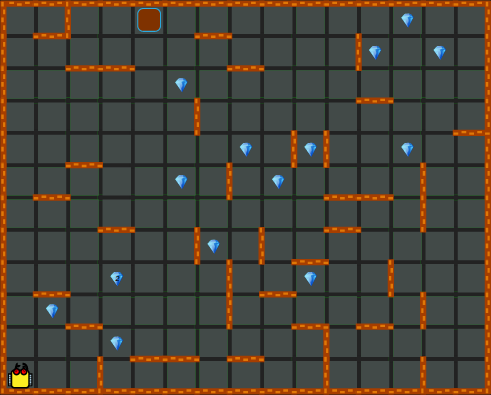
\includegraphics[height=0.4\textwidth]{img/gps-100.png}
\vspace{-0mm}
\caption{South-west corner of the maze has GPS coordinates [0, 0].}
\vspace{-6mm}
\label{fig:gps-100}
\end{center}
\end{figure}
\noindent
the above program will have the following output:\\

\begin{ybox}
\begin{verbatim}
Horizontal position: 0
Vertical position: 0
\end{verbatim}
\end{ybox}
\vspace{6mm}

\noindent
The maze's width (in west-east direction) is 15 tiles, and its height (in south-north direction) 
is 12 tiles. If Karel stands in the north-east corner as shown in Fig. \ref{fig:gps-101},

\begin{figure}[!ht]
\begin{center}
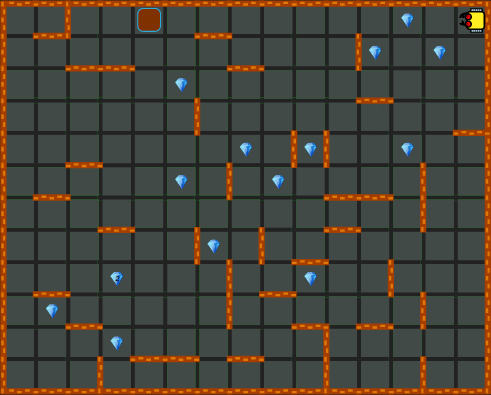
\includegraphics[height=0.4\textwidth]{img/gps-101.png}
\vspace{-0mm}
\caption{North-east corner of the maze has GPS coordinates [14, 11].}
%\vspace{-1cm}
\label{fig:gps-101}
\end{center}
\end{figure}

\noindent
then the output of the program is\\

\begin{ybox}
\begin{verbatim}
Horizontal position: 14
Vertical position: 11
\end{verbatim}
\end{ybox}
\vspace{6mm}

\noindent
Try to move Karel to other parts of the maze via simple commands or in Designer, 
and run the program again, to make yourself familiar with how the GPS device works.\\

\noindent
The {\tt print} command can be used to display more complicated sentences where text
and variables are separated by commas:\\

\begin{bbox}
\begin{Verbatim}[commandchars=\\\{\}]
\PY{k}{print} \PY{l+s}{"}\PY{l+s}{My GPS coordinates are}\PY{l+s}{"}\PY{p}{,} \PY{n}{gpsx}, \PY{l+s}{"and"}, \PY{n}{gpsy}
\end{Verbatim}
\end{bbox}
\vspace{6mm}

\noindent
Notice that each comma means the inclusion of one empty character:


\subsection[\ \ Defining custom functions]{Defining custom functions}

In Level 3 we can use the reserved word {\tt return} inside the body of
a command to return a value. Such commands are then called {\em functions}. 
They are also defined using the keyword {\tt def}. For example, the following function
{\tt count\_steps} will return the number of steps the robot needed to 
make in order to reach the closest wall in the direction that he was facing:\\

\begin{bbox}
\begin{Verbatim}[commandchars=\\\{\}]
\PY{k}{def} count_steps
    n = 0
    \PY{k}{while} \PY{n+nb+bp}{not} \PY{n+nb+bp}{wall}
        \PY{n+nf}{go}
        \PY{n+nf}{inc}(n)
    \PY{k}{return} n
\end{Verbatim}
\end{bbox}
\vspace{6mm}

\noindent
Notice couple of things here:
\begin{itemize}
\item The variable {\tt n} was created and initialized by {\tt 0} using {\tt n = 0}. In
      Karel, we do not have to state the type of a variable in advance -- the interpreter 
      will figure it out from the type of value that is first assigned to it.  
\item The {\tt inc()} function increases the value of an integer variable by one. 
      There is also a function {\tt dec()}, not used in the above program, that decreases 
      the value of an integer variable by one. More about these two functions will be said 
      in Paragraph \ref{subsec:incdec}.
\end{itemize}
The function can then be used as follows:\\

\begin{bbox}
\begin{Verbatim}[commandchars=\\\{\}]
\PY{n}{num} \PY{o}{=} \PY{n}{count\PYZus{}steps}
\PY{k}{print} \PY{l+s}{"}\PY{l+s}{Number of steps:}\PY{l+s}{"}\PY{p}{,} \PY{n}{num} 
\end{Verbatim}
\end{bbox}
\vspace{6mm}

\noindent
Here, we create a new variable {\tt num} and initialize it using the 
integer value that is returned by the {\tt count\_steps} function.
The result is then printed. For the situation shown in Fig. \ref{fig:cf-1},
\newpage

\begin{figure}[!ht]
\begin{center}
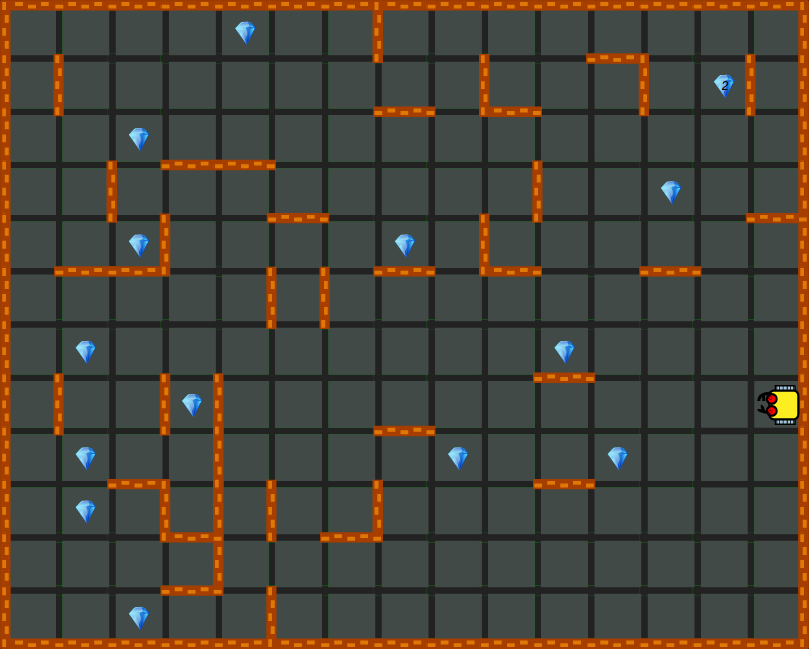
\includegraphics[height=0.4\textwidth]{img/maze-new-1.png}
\vspace{-0mm}
\caption{Testing the function {\tt count\_steps}.}
\vspace{-1cm}
\label{fig:cf-1}
\end{center}
\end{figure}

\noindent
the output is\\

\begin{ybox}
\begin{verbatim}
Number of steps: 10
\end{verbatim}
\end{ybox}
\vspace{6mm}
\subsection[\ \ Creating and initializing numerical variables]{Creating and initializing numerical variables} \label{par:var}

In Karel, numerical variables can be created and initialized in several different ways: 
\begin{enumerate}
\item By setting them to an integer number. For example, new variable {\tt a} is created and set to zero by typing \\

\begin{bboxshort}
\begin{Verbatim}[commandchars=\\\{\}]
a = 0
\end{Verbatim}
\end{bboxshort}
\vspace{1mm}

\noindent
\item By setting them to {\tt gpsx}. For example, new variable {\tt var} is created and set to {\tt gpsx} by typing\\

\begin{bboxshort}
\begin{Verbatim}[commandchars=\\\{\}]
var = gpsx
\end{Verbatim}
\end{bboxshort}
\vspace{1mm}

\noindent
\item By setting them to {\tt gpsy}. For example, new variable {\tt pos1} is created and set to {\tt gpsy} by typing\\

\begin{bboxshort}
\begin{Verbatim}[commandchars=\\\{\}]
pos1 = gpsy
\end{Verbatim}
\end{bboxshort}
\vspace{1mm}

\noindent
\item Initialize them with an existing value. For example, if there already is an integer variable 
{\tt var1}, then a new variable {\tt var2} can be created as follows:\\

\begin{bboxshort}
\begin{Verbatim}[commandchars=\\\{\}]
var2 = var1
\end{Verbatim}
\end{bboxshort}
\vspace{1mm}

\noindent
\item Initialize them with value returned by an existing function, as it was shown 
with the function {\tt count\_steps} in the previous paragraph:\\

\begin{bbox}
\begin{Verbatim}[commandchars=\\\{\}]
\PY{n}{num} \PY{o}{=} \PY{n}{count\PYZus{}steps}
\end{Verbatim}
\end{bbox}
\end{enumerate}

\subsection[\ \ Changing values of numerical variables]{Changing values of numerical variables}

The value of a numerical variable can be updated at any time by redefining it via 
one of the five options described in the previous paragraph. For example, let's say that 
Karel stands as shown in Fig. \ref{fig:var1}.

\begin{figure}[!ht]
\begin{center}
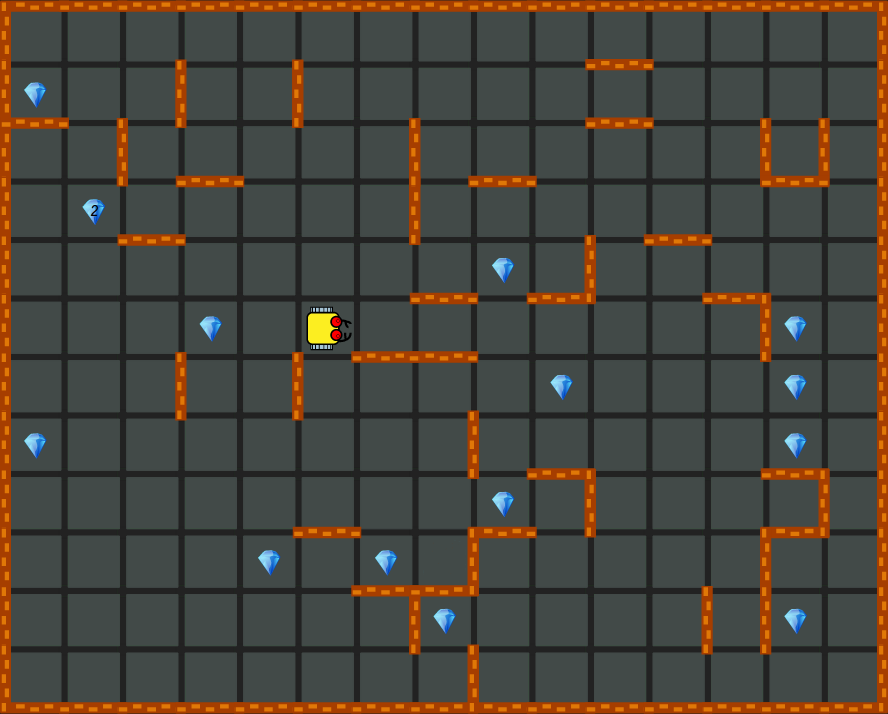
\includegraphics[height=0.4\textwidth]{img/variables1.png}
\end{center}
\vspace{-4mm}
\caption{Karel's initial position.}
\label{fig:var1}
%\vspace{-1cm}
\end{figure}

\noindent
Then the program\\

\begin{bbox}
\begin{Verbatim}[commandchars=\\\{\}]
a = gpsx
\PY{k}{print} \PY{l+s}{"Start position:"}, a
\PY{k}{repeat} 5
    \PY{n+nf}{go}
a = gpsx 
\PY{k}{print} \PY{l+s}{"End position:"}, a
\end{Verbatim}
\end{bbox}
\vspace{6mm}

\noindent
will produce the following output:\\

\begin{ybox}
\begin{verbatim}
Start position: 5
End position: 10
\end{verbatim}
\end{ybox}
\vspace{6mm}

\subsection[\ \ Using functions {\tt inc()} and {\tt dec()}]{Using functions {\tt inc()} and {\tt dec()}}\label{subsec:incdec}

As we saw before, we can increase or decrease the value of a numerical 
variable by one using the functions {\tt inc()} and 
{\tt dec()}, respectively. The full version of these functions 
is {\tt inc(n, num)} and {\tt dec(n, num)} where {\tt n} is the 
name of the variable and {\tt num} is 
an integer number that is set to one by default.

Consider again Karel's initial position as shown 
in Fig. \ref{fig:var1}. Then the code\\

\begin{bbox}
\begin{Verbatim}[commandchars=\\\{\}]
a = 0
\PY{k}{while} \PY{n+nb+bp}{not} \PY{n+nb+bp}{wall}
    \PY{n+nf}{go}
    \PY{n+nf}{inc}(a)
\PY{n+nf}{print} \PY{l+s}{"Went"}, a, \PY{l+s}{"steps before reaching a wall."}
\end{Verbatim}
\end{bbox}
\vspace{6mm}

\noindent
will have the following output:\\

\begin{ybox}
\begin{verbatim}
Went 7 steps before reaching a wall.
\end{verbatim}
\end{ybox}
\vspace{6mm}

\subsection[\ \ Comparison operations]{Comparison operations}

Integer numbers and numerical variables can be compared using the 
standard operators {\tt >, <, >=, <=, ==, !=, <>}. In this order, 
they read "greater than", "less than", "greater than or equal to", 
"less than or equal to", "equal to", "not equal to" and "not equal to"
(the last two operations have the same meaning). The result of each such 
operation is a logical value {\tt True} or {\tt False}, and it can be 
either used in a condition or conditional loop, or assigned to 
a variable. For example,\\

\begin{bbox}
\begin{Verbatim}[commandchars=\\\{\}]
a = 1
b = 5
\PY{k}{print} a < b
\end{Verbatim}
\end{bbox}
\vspace{6mm}

\noindent
yields the output\\

\begin{ybox}
\begin{Verbatim}[commandchars=\\\{\}]
True
\end{Verbatim}
\end{ybox}
\vspace{6mm}

\noindent
The code\\

\begin{bbox}
\begin{Verbatim}[commandchars=\\\{\}]
a = 1
b = 5
c = a > b
\PY{k}{print} c
\end{Verbatim}
\end{bbox}
\vspace{6mm}

\noindent
yields\\

\begin{ybox}
\begin{Verbatim}[commandchars=\\\{\}]
False
\end{Verbatim}
\end{ybox}
\vspace{6mm}

\noindent
The code \\

\begin{bbox}
\begin{Verbatim}[commandchars=\\\{\}]
a = 0
\PY{k}{while} a <= 5
  \PY{k}{print} a 
  \PY{n+nf}{inc}(a)
\end{Verbatim}
\end{bbox}
\vspace{6mm}

\noindent
yields\\

\begin{ybox}
\begin{Verbatim}[commandchars=\\\{\}]
0
1
2
3
4
5
\end{Verbatim}
\end{ybox}
\vspace{6mm}

\noindent

\subsection[\ \ Text string variables]{Text string variables}

Text string variables are created and initialized analogously 
to numerical variables:\\

\begin{bbox}
\begin{Verbatim}[commandchars=\\\{\}]
robot_name = \PY{s+1}{"Karel"}
\end{Verbatim}
\end{bbox}
\vspace{6mm}
 
\noindent
They can be printed as usual. The code\\

\begin{bbox}
\begin{Verbatim}[commandchars=\\\{\}]
\PY{k}{print} \PY{s+1}{"Robot's name is"}, my_name
\end{Verbatim}
\end{bbox}
\vspace{6mm}

\noindent
yields\\

\begin{ybox}
\begin{Verbatim}[commandchars=\\\{\}]
MRobot's name is Karel
\end{Verbatim}
\end{ybox}
\vspace{6mm}

\noindent
A text string variable can be used to initialize a new one. Let's say 
that someone wants to rename the robot to "Carlos" (which is the Spanish 
version of "Karel"),
and store his original name in the variable {\tt robot\_name\_orig}. 
This is done as follows:\\

\begin{bbox}
\begin{Verbatim}[commandchars=\\\{\}]
robot_name_orig = robot_name
robot_name = \PY{s+1}{"Carlos"}
\end{Verbatim}
\end{bbox}
\vspace{6mm}

\noindent
Text string variables can be useful, for example, to store texts for 
error messages and warnings in larger programs. Then, they can be 
defined in one place, although they are used in many different parts of 
the program. When we need to change such error message, we can do it 
very elegantly where the variable is defined, without having to go through 
the entire program and change the text everywhere.  

\subsection[\ \ Local and global variables]{Local and global variables}\label{subsec:karellocvar}

Note that a variable that is defined inside a function is {\em local to that function}, 
meaning that it can be used in the function only. If we attempt to use it 
outside, an error is thrown. For illustration, the code \\

\begin{bbox}
\begin{Verbatim}[commandchars=\\\{\}]
\PY{k}{def} myfunction
  a = 1

myfunction
\PY{k}{print} a  
\end{Verbatim}
\end{bbox}
\vspace{6mm}

\noindent
throws an error message \\

\begin{ybox}
\begin{Verbatim}[commandchars=\\\{\}]
\PY{s+1}{Unknown variable/procedure "a"} 
\end{Verbatim}
\end{ybox}
\vspace{6mm}

\noindent
Although using local variables might seem constraining, in reality it helps us 
to keep our code fit. It is a very good habit to keep variables in our programs 
as local as possible. More about local and global variables will be said in 
the Python textbook.

\section{Lists}

In this Section we introduce the concept of a {\em list}. 
The syntax and philosophy is the same as in the Python programming 
language, so all you learn here is directly usable in Python.
The Python language provides additional functionality for
working with lists which is not covered in Karel.

\subsection[\ \ Objectives]{Objectives} 
 
\begin{itemize}
\item Understand the concept of a list.
\item Learn to create empty lists, add items, and delete items.
\item Learn to parse lists and work with indices.
\end{itemize}
Lists are very useful data structures that can be used to store multiple 
integer values, logical values, or text strings at the same time. 
Values of different types can be combined and lists can even contain other lists.
Objects in a list are ordered and they can be added to the end of a list, 
accessed by their index, and deleted from any position of the list. Let us 
illustrate this functionality on examples.

\subsection[\ \ Creating a list]{Creating a list}

\noindent
An empty list {\tt U} is created via \\

\begin{bbox}
\begin{Verbatim}[commandchars=\\\{\}]
U = []
\end{Verbatim}
\end{bbox}
\vspace{6mm}

\noindent
Lists can be also created non-empty:\\

\begin{bbox}
\begin{Verbatim}[commandchars=\\\{\}]
V = [1, 2, 3, 4, 5]
\end{Verbatim}
\end{bbox}
\vspace{6mm}

\noindent
One can use variables when creating a list:\\

\begin{bbox}
\begin{Verbatim}[commandchars=\\\{\}]
c = 100
W = [0, 50, c]
\PY{k}{print} W
\end{Verbatim}
\end{bbox}
\vspace{6mm}

\noindent
whose output is \\

\begin{ybox}
\begin{Verbatim}[commandchars=\\\{\}]
[0, 50, 100]
\end{Verbatim}
\end{ybox}
\vspace{6mm}

\noindent
Integer numbers can be combined with text strings:\\

\begin{bbox}
\begin{Verbatim}[commandchars=\\\{\}]
X = [1, \PY{s+1}{"Hello"}, 2]
\end{Verbatim}
\end{bbox}
\vspace{6mm}

\noindent
Lists can contain other lists as their elements:\\

\begin{bbox}
\begin{Verbatim}[commandchars=\\\{\}]
Y = [1, \PY{s+1}{"Hello"}, 2, [1, 2, 3]]
\end{Verbatim}
\end{bbox}
\vspace{6mm}

\noindent
One can print a list as expected:\\

\begin{bbox}
\begin{Verbatim}[commandchars=\\\{\}]
\PY{k}{print} \PY{s+1}{"This is the list Y:"}, Y
\end{Verbatim}
\end{bbox}
\vspace{6mm}

\noindent
Output:\\

\begin{ybox}
\begin{Verbatim}[commandchars=\\\{\}]
This is the list Y: [1, \PY{s+1}{"Hello"}, 2, [1, 2, 3]]
\end{Verbatim}
\end{ybox}
\vspace{6mm}

\subsection[\ \ Accessing list items by their index]{Accessing list items by their index}

\noindent
Any list item can be accessed and either printed, assigned 
to a variable, or used in an operation, via its index. Indices 
always start from zero. In other words, {\tt L[0]} is the 
first item in the list {\tt L}, {\tt L[1]} is the second one, etc. 
Working with indices can be illustrated using a simple code\\

\begin{bbox}
\begin{Verbatim}[commandchars=\\\{\}]
L = [8, 12, 16, 20]
\PY{k}{print} \PY{s+1}{"First item:"}, L[0]
\PY{k}{print} \PY{s+1}{"Second item:"}, L[1]
\PY{k}{print} \PY{s+1}{"Third item:"}, L[2]
\PY{k}{print} \PY{s+1}{"Fourth item:"}, L[3]
\end{Verbatim}
\end{bbox}
\vspace{6mm}

\noindent
whose output is\\

\begin{ybox}
\begin{Verbatim}[commandchars=\\\{\}]
First item: 8
Second item: 12
Third item: 16
Fourth item: 20
\end{Verbatim}
\end{ybox}
\vspace{6mm}

\subsection[\ \ Appending items to a list]{Appending items to a list}

\noindent
An arbitrary object {\tt obj} (integer, text string, logical value, another list, etc.) can be appended 
to the end of an existing list using the {\tt append()} function. For a list {\tt L} this would be\\

\begin{bbox}
\begin{Verbatim}[commandchars=\\\{\}]
L.append(obj)
\end{Verbatim}
\end{bbox}
\vspace{6mm}

\noindent
For illustration, the code\\

\begin{bbox}
\begin{Verbatim}[commandchars=\\\{\}]
K = [1, 11]
K.append(21)
\PY{k}{print} K
\end{Verbatim}
\end{bbox}
\vspace{6mm}

\noindent
has the output\\

\begin{ybox}
\begin{Verbatim}[commandchars=\\\{\}]
[1, 11, 21]
\end{Verbatim}
\end{ybox}
\vspace{6mm}

\subsection[\ \ Removing items via the {\tt pop()} function]{Removing items via the {\tt pop()} function}

\noindent
The {\tt i}th item (where indices start from zero) can be deleted 
from a list {\tt L} and assigned to a variable {\tt x} via \\

\begin{bbox}
\begin{Verbatim}[commandchars=\\\{\}]
x = L.pop(i)
\end{Verbatim}
\end{bbox}
\vspace{6mm}

\noindent
For illustration, let us create a list {\tt X} containing 
three text strings "Monday", "Tuesday" and "Wednesday", and then
delete the second item:\\

\begin{bbox}
\begin{Verbatim}[commandchars=\\\{\}]
X = ["Monday", "Tuesday", "Wednesday"]
day = X.pop(1)
print day
print X
\end{Verbatim}
\end{bbox}
\vspace{6mm}

\noindent
The output of this code is\\

\begin{ybox}
\begin{Verbatim}[commandchars=\\\{\}]
Tuesday
['Monday', 'Wednesday']
\end{Verbatim}
\end{ybox}
\vspace{6mm}

\noindent
If the {\tt pop()} function is used without an index, it removes
and returns the last object of the list:\\

\begin{bbox}
\begin{Verbatim}[commandchars=\\\{\}]
day = X.pop()
print day
print X
\end{Verbatim}
\end{bbox}
\vspace{6mm}

\noindent
Output:\\

\begin{ybox}
\begin{Verbatim}[commandchars=\\\{\}]
Wednesday
['Monday']
\end{Verbatim}
\end{ybox}
\vspace{6mm}

\subsection[\ \ Deleting items via the {\tt del} command]{Deleting items via the {\tt del} command}

\noindent
The purpose of the {\tt del} command is similar to the {\tt pop()} function
except that the deleted object is destroyed (it cannot be assigned to a variable).
The {\tt i}th item can be deleted from a list {\tt L} via \\

\begin{bbox}
\begin{Verbatim}[commandchars=\\\{\}]
\PY{n+nf}{del} L[i]
\end{Verbatim}
\end{bbox}
\vspace{6mm}

\noindent
For illustration, the output of the code \\

\begin{bbox}
\begin{Verbatim}[commandchars=\\\{\}]
L = ["Monday", "Tuesday", "Wednesday"]
\PY{n+nf}{del} L[0]
\PY{k}{print} L
\PY{n+nf}{del} L[0]
\PY{k}{print} L
\end{Verbatim}
\end{bbox}
\vspace{6mm}

\noindent
is \\

\begin{ybox}
\begin{Verbatim}[commandchars=\\\{\}]
['Tuesday', 'Wednesday']
['Wednesday']
\end{Verbatim}
\end{ybox}
\vspace{6mm}

\subsection[\ \ Length of a list]{Length of a list}

\noindent
The function {\tt len(X)} returns the length of the list {\tt X}.
For illustration, the code \\

\begin{bbox}
\begin{Verbatim}[commandchars=\\\{\}]
M = [\PY{s+1}{"John"}, \PY{s+1}{"Josh"}, \PY{s+1}{"Jim"}, \PY{s+1}{"Jane"}]
n = \PY{n+nf}{len}(L)
\PY{k}{print} \PY{s+1}{"Length of the list is"}, n
\end{Verbatim}
\end{bbox}
\vspace{6mm}

\noindent
has the output\\

\begin{ybox}
\begin{Verbatim}[commandchars=\\\{\}]
Length of the list is 4
\end{Verbatim}
\end{ybox}
\vspace{6mm}

\subsection[\ \ Parsing lists]{Parsing lists}

In Karel, lists can be parsed via the {\tt repeat} command.
For illustration, the following sample code defines a list {\tt M} consisting of four numbers 
{\tt 1, 2, 3, 4} and prints all of them increased by two: \\

\begin{bbox}
\begin{Verbatim}[commandchars=\\\{\}]
M = [1, 3, 5, 7]
n = \PY{n+nf}{len}(L)
i = 0
\PY{k}{repeat} n
    c = M[i]
    \PY{k}{print} \PY{n+nf}{inc}(c, 2)
    \PY{n+nf}{inc}(i)
\end{Verbatim}
\end{bbox}
\vspace{6mm}

\subsection[\ \ Storing the robot's path in a list]{Storing the robot's path in a list}

\noindent
Lists can be used to store the robot's path. The following 
is a simple program that only tells the robot to go straight to the 
nearest wall (this part does not really matter) and store the GPS
coordinates in a list {\tt L}:\\

\begin{bbox}
\begin{Verbatim}[commandchars=\\\{\}]
L = []
\PY{k}{while} \PY{n+nb+bp}{not} \PY{n+nb+bp}{wall}
    L.append([gpsx, gpsy])
    \PY{n+nf}{go}
L.append([gpsx, gpsy])
\PY{k}{print} \PY{s+1}{"Path: "}, L
\end{Verbatim}
\end{bbox}
\vspace{6mm}

\noindent
In fact, each time we are appending a list consisting of the horizontal and 
vertical GPS coordinates -- there is no other way to represent two numbers 
in one variable unless the variable is a list. When the robot's initial position 
is as shown in Fig. \ref{fig:list-1},
\newpage

\begin{figure}[!ht]
\begin{center}
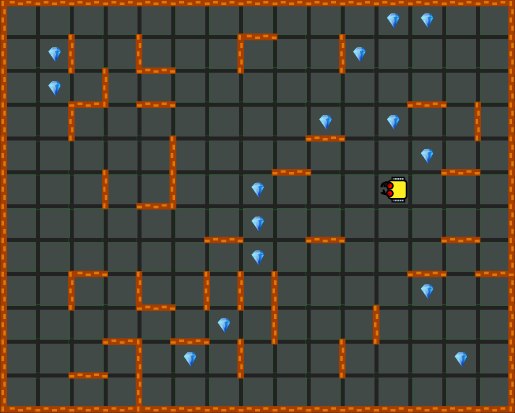
\includegraphics[height=0.4\textwidth]{img/lists-1.png}
\vspace{-0mm}
\caption{Robot stands at position [11, 6] facing west.}
%\vspace{-1cm}
\label{fig:list-1}
\end{center}
\end{figure}

\noindent
then the output of the above program is\\

\begin{ybox}
\begin{Verbatim}[commandchars=\\\{\}]
Path: [[11, 6], [10, 6], [9, 6], [8, 6], [7, 6], [6, 6], 
[5, 6]]
\end{Verbatim}
\end{ybox}
\vspace{6mm}

\noindent
To keep Karel's language simple, we do not allow double indices. Nevertheless
there is a simple way to get to the items of lists that are contained in other lists:\\

\begin{bbox}
\begin{Verbatim}[commandchars=\\\{\}]
a = L[0]
\PY{k}{print} \PY{s+1}{"Horizontal coordinate of initial position:"}, a[0]
\PY{k}{print} \PY{s+1}{"Vertical coordinate of initial position:"}, a[1]
a = L[1]
\PY{k}{print} \PY{s+1}{"Horizontal coordinate after one step:"}, a[0]
\PY{k}{print} \PY{s+1}{"Vertical coordinate after one step:"}, a[1]
...
\end{Verbatim}
\end{bbox}

%%%%%%%%%%%%%%%%%%%%%%%%%%%%%%%%%%%%%%%%%%%%%%%%%%%%%%%%%%%%%%%%%%%%%%%%%%%%%%%

\section{Logic} \label{sec:logic} 

\subsection[\ \ Objectives]{Objectives} 
 
\begin{itemize}
\item Review elementary logic.
\item Practice working with more complex logical expressions.
\end{itemize}

\subsection[\ \ Simple logical expressions]{Simple logical expressions}

As we already know, logical expressions are expressions that can be answered with either {\tt True} or 
{\tt False}. We say that the {\tt True} or the {\tt False} is their {\em value}. Here are some 
real-life examples, try to answer them with {\tt True} or {\tt False}:

\begin{itemize}
\item "I am 15 years old."
\item "My dad is a teacher."
\item "My school's name is Coral Academy."
\end{itemize}
And here are some Karel examples:
\begin{itemize}
\item {\color{ForestGreen} \tt wall} ... {\tt True} if the robot is facing a wall, {\tt False} otherwise.
\item {\color{ForestGreen} \tt gem}  ... {\tt True} if the robot stands on a gem, {\tt False} otherwise.
\item {\color{ForestGreen} \tt north} ... {\tt True} if the robot is facing North, {\tt False} otherwise.
\item {\color{ForestGreen} \tt home} ... {\tt True} if the robot is home, {\tt False} otherwise.
\item {\color{ForestGreen} \tt empty} ... {\tt True} if the robot does not have any gems on him, {\tt False} otherwise.
\end{itemize}
Let's consider the situation shown in Fig. \ref{fig:logic1}.

\begin{figure}[!ht]
\begin{center}
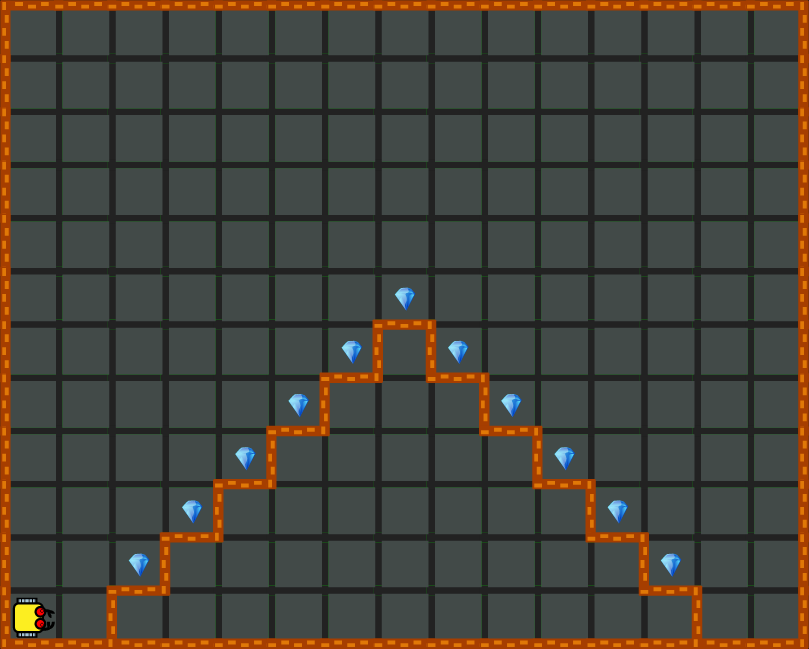
\includegraphics[width=0.7\textwidth]{img/logic-1.png}
\end{center}
\vspace{-2mm}
\caption{Karel is testing the {\tt wall} sensor.}
\label{fig:logic1}
%\vspace{-10mm}
\end{figure}
\noindent
The following code shows different ways we can operate with the 
logical value provided by the {\tt wall} sensor:\\

\begin{bbox}
\begin{Verbatim}[commandchars=\\\{\}]
\PY{n+nb+bp}{wall}
\PY{k}{print} \PY{s+1}{"Value of the wall sensor:"}, \PY{n+nb+bp}{wall}
value = \PY{n+nb+bp}{wall}
\PY{k}{if} value
    \PY{k}{print} \PY{s+1}{"I am standing in front of a wall."}
\PY{k}{else}
    \PY{k}{print} \PY{s+1}{"There is no wall in front of me."}
\end{Verbatim}
\end{bbox}
\vspace{6mm}

\noindent
The output of this code is \\

\begin{ybox}
\begin{Verbatim}[commandchars=\\\{\}]
False
Value of the wall sensor: False
There is no wall in front of me.
\end{Verbatim}
\end{ybox}

\subsection[\ \ Complex logical expressions]{Complex logical expressions}

In programming as well as in real life we often deal with logical expressions that are 
fairly complex. Often we use two or more simple logical expressions in one sentence, 
and moreover combine them with logical operations {\tt and}, {\tt or} or {\tt not}.

For example, the sentence "I will go skiing on Saturday if weather is good and if 
Michael goes as well." includes three simple logical expressions. Let's call 
them for brevity\\

\noindent
{\tt A} = "I will go skiing on Saturday."\\
{\tt B} = "The weather is good."\\
{\tt C} = "Michael goes as well."\\

\noindent
There is a logical operation {\tt and} between the expressions {\tt B}, {\tt C}.
The original sentence can be written briefly as \\

\centerline{
if {\tt B} {\tt and} {\tt C} then {\tt A}
}
\vspace{4mm}
\noindent
We love this kind of brevity in programming. Let's say that we can 
predict the future and we know that the weather will be good and that 
Michael will go as well. Then we can translate the above condition 
into computer code. We also print the resulting value of {\tt A}
at the end:\\

\begin{bbox}
\begin{Verbatim}[commandchars=\\\{\}]
\PY{c}{\PYZsh{} Let's say that weather will be good}
\PY{c}{\PYZsh{} and Michael will join you:}
B = \PY{n+nb+bp}{True}
C = \PY{n+nb+bp}{True}
\PY{c}{\PYZsh{} This is how you decide:}
\PY{k}{if} B and C
    A = \PY{n+nb+bp}{True}
\PY{k}{else}
    A = \PY{n+nb+bp}{False}
\PY{c}{\PYZsh{} Print the result:}
\PY{k}{if} A
    \PY{k}{print} \PY{s+1}{"I will go ski on Sunday."}
\PY{k}{else}
    \PY{k}{print} \PY{s+1}{"I will not go ski on Sunday."}
\end{Verbatim}
\end{bbox}
\vspace{6mm}

\noindent
Output:\\

\begin{ybox}
\begin{Verbatim}[commandchars=\\\{\}]
I will go ski on Sunday.
\end{Verbatim}
\end{ybox}

\subsection[\ \ Truth tables]{Truth tables}

Each of these three logical operations comes with its own {\em truth table} that 
summarizes its results for different values of operands. The truth table for the 
logical {\tt and} is:\\

\begin{center}
\begin{tabular}{|c|c||c|}
\hline
{\tt A} & {\tt B} & \ {\tt A} {\tt and} {\tt B} \ \\
\hline
\hline
{\tt True} & {\tt True} & {\tt True} \\
\hline
{\tt True} & \ {\tt False} \ & \ {\tt False} \ \\
\hline
\ {\tt False} \ & {\tt True} & \ {\tt False} \ \\
\hline
\ {\tt False} \ & \ {\tt False} \ & \ {\tt False} \ \\
\hline
\end{tabular}
\end{center}
\vspace{4mm}
\noindent
The truth table for logical {\tt or} is:\\

\begin{center}
\begin{tabular}{|c|c||c|}
\hline
{\tt A} & {\tt B} & \ {\tt A} {\tt or} {\tt B} \ \\
\hline
\hline
{\tt True} & {\tt True} & {\tt True} \\
\hline
{\tt True} & \ {\tt False} \ & \ {\tt True} \ \\
\hline
\ {\tt False} \ & {\tt True} & \ {\tt True} \ \\
\hline
\ {\tt False} \ & \ {\tt False} \ & \ {\tt False} \ \\
\hline
\end{tabular}
\end{center}
\vspace{4mm}
\noindent
And finally, truth table for logical {\tt not} is:\\

\begin{center}
\begin{tabular}{|c||c|}
\hline
{\tt A} & \ {\tt not} {\tt A} \ \\
\hline
\hline
{\tt True} & {\tt False} \\
\hline
{\tt False} & \ {\tt True} \ \\
\hline
\end{tabular}
\end{center}
\vspace{4mm}
\noindent

%%%%%%%%%%%%%%%%%%%%%%%%%%%%%%%%%%%%%%%%%%%%%%%%%%%%%%%%%%%%%%%%%%%%%%%%%%%%%%%

\section{Appendix - Overview of Functionality by Level}\label{sec:newfunc3}

\subsection[\ \ Level 0 (Section \ref{sec:manual})]{Level 0 (Section \ref{sec:manual})}

In Level 0, Karel can be guided by clicking on buttons:
\begin{itemize}
\item Go ... make one step forward.
\item Left ... turn left.
\item Right ... turn right.
\item Put ... put a gem on the ground.
\item Get ... pick up a gem from the ground.
\end{itemize}

\subsection[\ \ Level 1 (Section \ref{sec:bridge})]{Level 1 (Section \ref{sec:bridge})}

In Level 1, Karel can be guided by typing the commands:
\begin{itemize}
\item {\tt go} ... make one step forward.
\item {\tt left} ... turn left.
\item {\tt right} ... turn right.
\item {\tt put} ... put a gem on the ground.
\item {\tt get} ... pick up a gem from the ground.
\end{itemize}

\subsection[\ \ Level 2 (Sections \ref{sec:repeat} -- \ref{sec:recursion})]{Level 2 (Sections \ref{sec:repeat} -- \ref{sec:recursion})}

New commands:
\begin{itemize}
\item {\tt if - else} ... condition.
\item {\tt repeat} ... counting loop (repeat an action a given number of times).
\item {\tt while} ... conditional loop (repeat an action while a condition is satisfied).
\item {\tt def} ... define a new command.
\end{itemize}
Additional new keywords:
\begin{itemize}
\item {\tt wall} ... sensor that checks True if the robot faces a wall.
\item {\tt gem} ... sensor that checks True if there is a gem within the robot's reach.
\item {\tt empty} ... sensor that checks True if the robot's bag with gems is empty.
\item {\tt home} ... sensor that checks True if the robot is at home.
\item {\tt north} ... sensor that checks True if the robot faces North.
\end{itemize}
New functionality:
\begin{itemize}
\item Recursion (a command can make a call to itself).
\end{itemize}

\subsection[\ \ Level 3 (Sections \ref{sec:var}, \ref{sec:logic})]{Level 3 (Sections \ref{sec:var}, \ref{sec:logic})}

New keywords:
\begin{itemize}
\item {\tt print} ... print strings and variables.
\item {\tt gpsx} ... GPS coordinate in the horizontal direction.
\item {\tt gpsy} ... GPS coordinate in the vertical direction.
\item {\tt a = 0} ... create a new variable {\tt a} and initialize it with zero (or another 
      integer number).\\ For additional ways to initialize variables see Subsection \ref{par:var}.
\item {\tt inc(a)} ... increases the value of variable {\tt a} by one.
\item {\tt inc(a, value)} ... increases the value of variable {\tt a} by {\tt value}.
\item {\tt dec(a)} ... decreases the value of variable {\tt a} by one.
\item {\tt dec(a, value)} ... decreases the value of variable {\tt a} by {\tt value}.
\item {\tt rand} ... random command (returns randomly True or False).
\item {\tt return} ... returns a value, to be used in functions.
\item {\tt and} ... binary logical {\em and}.
\item {\tt or} ... binary logical {\em or}.
\item {\tt not} ... unary logical {\em not}.
\item {\tt len(L)} ... length of list {\tt L}.
\item {\tt L[i]} ... object at position {\tt i} in list {\tt L}. Note: {\tt L[0]} is the first item in the list.
\item {\tt L.append(x)} ... appends {\tt x} to the end of list {\tt L}.
\item {\tt x = L.pop()} ... removes the last item of list {\tt L} and assigns it to {\tt x}.
\item {\tt del L[i]} ... removes from list {\tt L} object at position {\tt i}. 
\end{itemize}
New functionality:
\begin{itemize}
\item Numerical and logical (Boolean) variables.
\item Complex logical expressions.
\item Functions that return values.
\item Lists.
\end{itemize}


\section{What next?}

Congratulations, you made it through Karel the Robot! We hope that you 
enjoyed the textbook and exercises. If you can think of any way to 
improve the application Karel the Robot or this textbook, we would like
to hear from you. If you have an interesting new game or exercise for 
Karel, please let us know as well. 

You are now ready to dive into a next programming language! We would 
recommend Python which is a modern high-level dynamical programming 
language that is used in many diverse applications in business, science,
engineering, and other areas.\\

\noindent
In any case, our team wishes you good luck, and keep us in your 
favorite bookmarks! \\

\hbox{} \hfill{} Your Authors


